\documentclass{minimal}
\usepackage{epsfig,color}
\usepackage{units}
\usepackage[papersize={576.00bp,432.00bp},text={576.00bp,432.00bp}]{geometry}
\begin{document}
\centering
% Title: glps_renderer figure
% Creator: GL2PS 1.3.8, (C) 1999-2012 C. Geuzaine
% For: Octave
% CreationDate: Wed Oct 29 20:18:46 2014
\setlength{\unitlength}{1pt}
\begin{picture}(0,0)
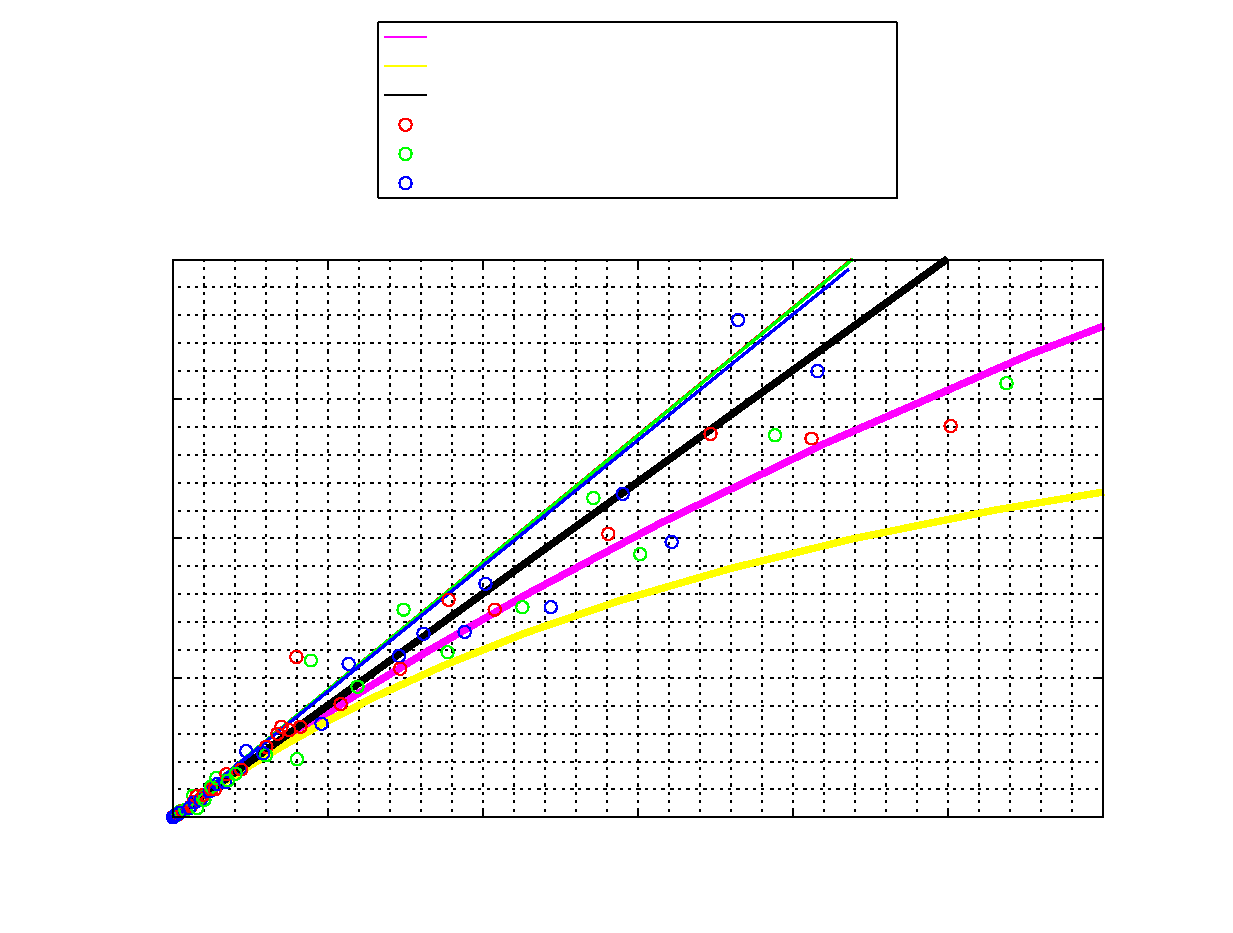
\includegraphics{gm-inc}
\end{picture}%
\begin{picture}(576,432)(0,0)
\fontsize{10}{0}
\selectfont\put(74.88,42.5252){\makebox(0,0)[t]{\textcolor[rgb]{0,0,0}{{0}}}}
\fontsize{10}{0}
\selectfont\put(149.28,42.5252){\makebox(0,0)[t]{\textcolor[rgb]{0,0,0}{{5}}}}
\fontsize{10}{0}
\selectfont\put(223.68,42.5252){\makebox(0,0)[t]{\textcolor[rgb]{0,0,0}{{10}}}}
\fontsize{10}{0}
\selectfont\put(298.08,42.5252){\makebox(0,0)[t]{\textcolor[rgb]{0,0,0}{{15}}}}
\fontsize{10}{0}
\selectfont\put(372.48,42.5252){\makebox(0,0)[t]{\textcolor[rgb]{0,0,0}{{20}}}}
\fontsize{10}{0}
\selectfont\put(446.88,42.5252){\makebox(0,0)[t]{\textcolor[rgb]{0,0,0}{{25}}}}
\fontsize{10}{0}
\selectfont\put(521.28,42.5252){\makebox(0,0)[t]{\textcolor[rgb]{0,0,0}{{30}}}}
\fontsize{10}{0}
\selectfont\put(69.8755,47.52){\makebox(0,0)[r]{\textcolor[rgb]{0,0,0}{{0}}}}
\fontsize{10}{0}
\selectfont\put(69.8755,114.45){\makebox(0,0)[r]{\textcolor[rgb]{0,0,0}{{0.2}}}}
\fontsize{10}{0}
\selectfont\put(69.8755,181.38){\makebox(0,0)[r]{\textcolor[rgb]{0,0,0}{{0.4}}}}
\fontsize{10}{0}
\selectfont\put(69.8755,248.31){\makebox(0,0)[r]{\textcolor[rgb]{0,0,0}{{0.6}}}}
\fontsize{10}{0}
\selectfont\put(69.8755,315.239){\makebox(0,0)[r]{\textcolor[rgb]{0,0,0}{{0.8}}}}
\fontsize{10}{0}
\selectfont\put(298.08,31.5252){\makebox(0,0)[t]{\textcolor[rgb]{0,0,0}{{$I_C [\unit{mA}]$}}}}
\fontsize{10}{0}
\selectfont\put(50.8755,181.38){\rotatebox{90}{\makebox(0,0)[b]{\textcolor[rgb]{0,0,0}{{$g_m [\unit{\Omega^{-1}}]$}}}}}
\fontsize{10}{0}
\selectfont\put(199.693,422.224){\makebox(0,0)[l]{\textcolor[rgb]{0,0,0}{{\texttt{PHIL\_BJT} $V_{th}= 26,14758\unit{mV}$}}}}
\fontsize{10}{0}
\selectfont\put(199.693,408.164){\makebox(0,0)[l]{\textcolor[rgb]{0,0,0}{{\texttt{SIEMENS} $V_{th}= 25,73160\unit{mV}$}}}}
\fontsize{10}{0}
\selectfont\put(199.693,394.104){\makebox(0,0)[l]{\textcolor[rgb]{0,0,0}{{modelo modificado $V_{th}= 25,78667\unit{mV}$}}}}
\fontsize{10}{0}
\selectfont\put(199.693,380.044){\makebox(0,0)[l]{\textcolor[rgb]{0,0,0}{{transistor 1 $V_{th}= 27,37242\unit{mV}$}}}}
\fontsize{10}{0}
\selectfont\put(199.693,365.984){\makebox(0,0)[l]{\textcolor[rgb]{0,0,0}{{transistor 2 $V_{th}= 27,40305\unit{mV}$}}}}
\fontsize{10}{0}
\selectfont\put(199.693,351.924){\makebox(0,0)[l]{\textcolor[rgb]{0,0,0}{{transistor 3 $V_{th}= 27,74140\unit{mV}$}}}}
\end{picture}
\end{document}
